



\begin{algorithm}[h]
\caption{\PyCode{Train(Data)}}
\begin{flushleft}
\PyInput{Input: Data=\{x0, x1\}} \\ 
\PyInput{Output: Model $v(x,t)$ for the rectified flow} \\ 
\PyCode{initialize Model} \\ 
\PyCode{for x0, x1 in Data:}
\PyComment{x0, x1:~samples from  $\tg_0$,  $\tg_1$} \\  %
\PyCode{~~~~Optimizer.zero\_grad()} \\
\PyCode{~~~~t = torch.rand(batchsize)}~~\PyComment{Randomly sample  $t \in$ [0,1]} \\
\PyCode{~~~~\blue{Loss = ( Model(t*x1+(1-t)*x0,~t) - (x1-x0) ).pow(2).mean()}} \\
\PyCode{~~~~Loss.backward()} \\
\PyCode{~~~~Optimizer.step()} \\
\PyCode{return Model} 
\end{flushleft}
\label{alg:pytorchAlgorithm}
\end{algorithm}


\begin{algorithm}[h]
\caption{\PyCode{Sample(Model, Data)}}
\begin{flushleft}
\PyInput{Input: Model $v(x,t)$ of the rectified flow} \\ 
\PyInput{Output: draws of the rectified coupling $(Z_0,Z_1)$} \\ 
\PyCode{coupling = []} \\
\PyCode{for x0, \_ in Data:}
\PyComment{x0:~samples from  $\tg_0$ (batchsize$\times$dim)} \\
\PyCode{~~~~x1 = model.ODE\_solver(x0)} \\
\PyCode{~~~~coupling.append((x0, x1))} \\
\PyCode{return coupling}
\end{flushleft}
\label{alg:rectify}
\end{algorithm}


\begin{algorithm}[h]
\caption{\PyCode{Reflow(Data)}}
\begin{flushleft}
\PyInput{Input: Data=\{x0, x1\}} \\ %
\PyInput{Output: draws of the $K$-th rectified coupling} \\ 
\PyCode{Coupling = Data} \\
\PyCode{for  $k=1,\ldots,K$:} \\ 
\PyCode{~~~~Model = Train(Coupling)}   \\
\PyCode{~~~~Coupling = sample(Model, Data)}   \\
\PyCode{return Coupling}
\end{flushleft}
\label{alg:rectify}
\end{algorithm}



\begin{figure}[h]%
  \begin{center}
  \begin{tabular}{lr}
    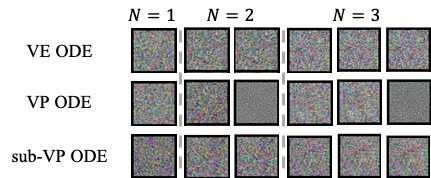
\includegraphics[width=0.45\textwidth]{arxiv_figures/flow_triangle_flatten/image_1.png}  &
    \smash{\raisebox{10pt}{ 
    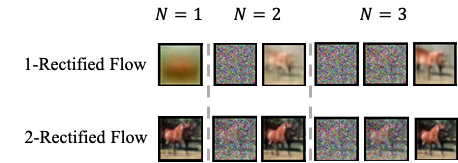
\includegraphics[width=0.45\textwidth]{arxiv_figures/flow_triangle_flatten/image_2.png} }
    }
    \end{tabular} 
  \end{center}
  \vspace{0\baselineskip}
  \caption{Few-step generation with different ODEs. Compared with VE,VP,sub-VP ODE, 1-rectified flow can generate blurry images using only 1,2,3 steps. After one time of rectification, 2-rectified flow can generate clear images with 1,2,3 steps. 
  }
  \label{fig:cifar10_triangle}
\end{figure}


\section{Additional Experiment Details}
\paragraph{Experiment Configuration on CIFAR10}  We conduct unconditional image generation with the CIFAR-10 dataset \citep{krizhevsky2009learning}. The resolution of the images are set to $32 \times 32$. For rectified flow, we adopt the same network structure as DDPM++ in \citep{song2020score}. The training of the network is smoothed by exponential moving average as in~\citep{song2020score}, with a ratio of $0.999999$. We adopt Adam~\citep{kingma2014adam} optimizer with a learning rate of $2e-4$ and a dropout rate of $0.15$.

For reflow, we first generate 4 million pairs of $(z_0, z_1)$ to get a new dataset $D$, then fine-tune the $i$-rectified flow model for $300,000$ steps to get the $(i+1)$-rectified flow model. We further distill these rectified flow models for few-step generation. To get a $k$-step image generator from the $i$-rectified flow, we randomly sample $t \in \{0, 1/k, \cdots, (k-1)/k\}$ during fine-tuning, instead of randomly sampling $t \in [0, 1]$. Specifically, for $k=1$, we replace the L2 loss function with the LPIPS similarity~\citep{zhang2018unreasonable} since it empirically brings better performance.

\paragraph{Expreiment Configuration on Image-to-Image Translation}
In this experiment, we also adopt the same U-Net structure of DDPM++~\cite{song2020score} for representing the drift $v^X$. 
We follow the procedure in Algorithm~\ref{alg:cap}. 
For the purpose of generative modeling, we set $\tg_0$ to be one domain dataset and $\tg_1$ the other domain dataset. 
For optimization, we use AdamW~\citep{loshchilov2017decoupled} optimizer with $\beta$ $(0.9, 0.999)$, weight decay $0.1$ and dropout rate $0.1$.
We train the model with a batch size of $4$ for $1,000$ epochs. 
We further apply exponential moving average (EMA) optimizer with coefficient $0.9999$.
We perform grid-search on the learning rate from $\{5\times 10^{-4}, 2\times 10^{-4}, 5\times 10^{-5}, 2\times 10^{-5}, 5\times 10^{-6}\}$ and pick the model with the lowest training loss.

We use the AFHQ \citep{choi2020stargan}, MetFace \citep{karras2020training} and CelebA-HQ \citep{karras2018progressive} dataset. 
Animal Faces HQ (AFHQ) is an animal-face dataset consisting of 15,000 high-quality images at $512 \times 512$ resolution. The dataset includes three domains of cat, dog, and wild animals, each providing 5000 images. 
MetFace consists of 1,336 high-quality PNG human-face images at $1024 \times 1024$ resolution, extracted from works of art.
CelebA-HQ is a human-face dataset which consists of 30,000 images at $1024 \times 1024$ resolution.
We randomly select $80\%$ as the training data and regard the rest as the test data, and resize the image to $512 \times 512$.

\paragraph{Experiment Configuration on Domain Adaptation}
For training the model, we apply AdamW~\citep{loshchilov2017decoupled} optimizer with batch size $16$, number of iterations $50$k, learning rate $10^{-4}$, weight decay $0.1$ and OneCycle \citep{smith2019onecycle} learning rate schedule.

\begin{figure}
    \centering
    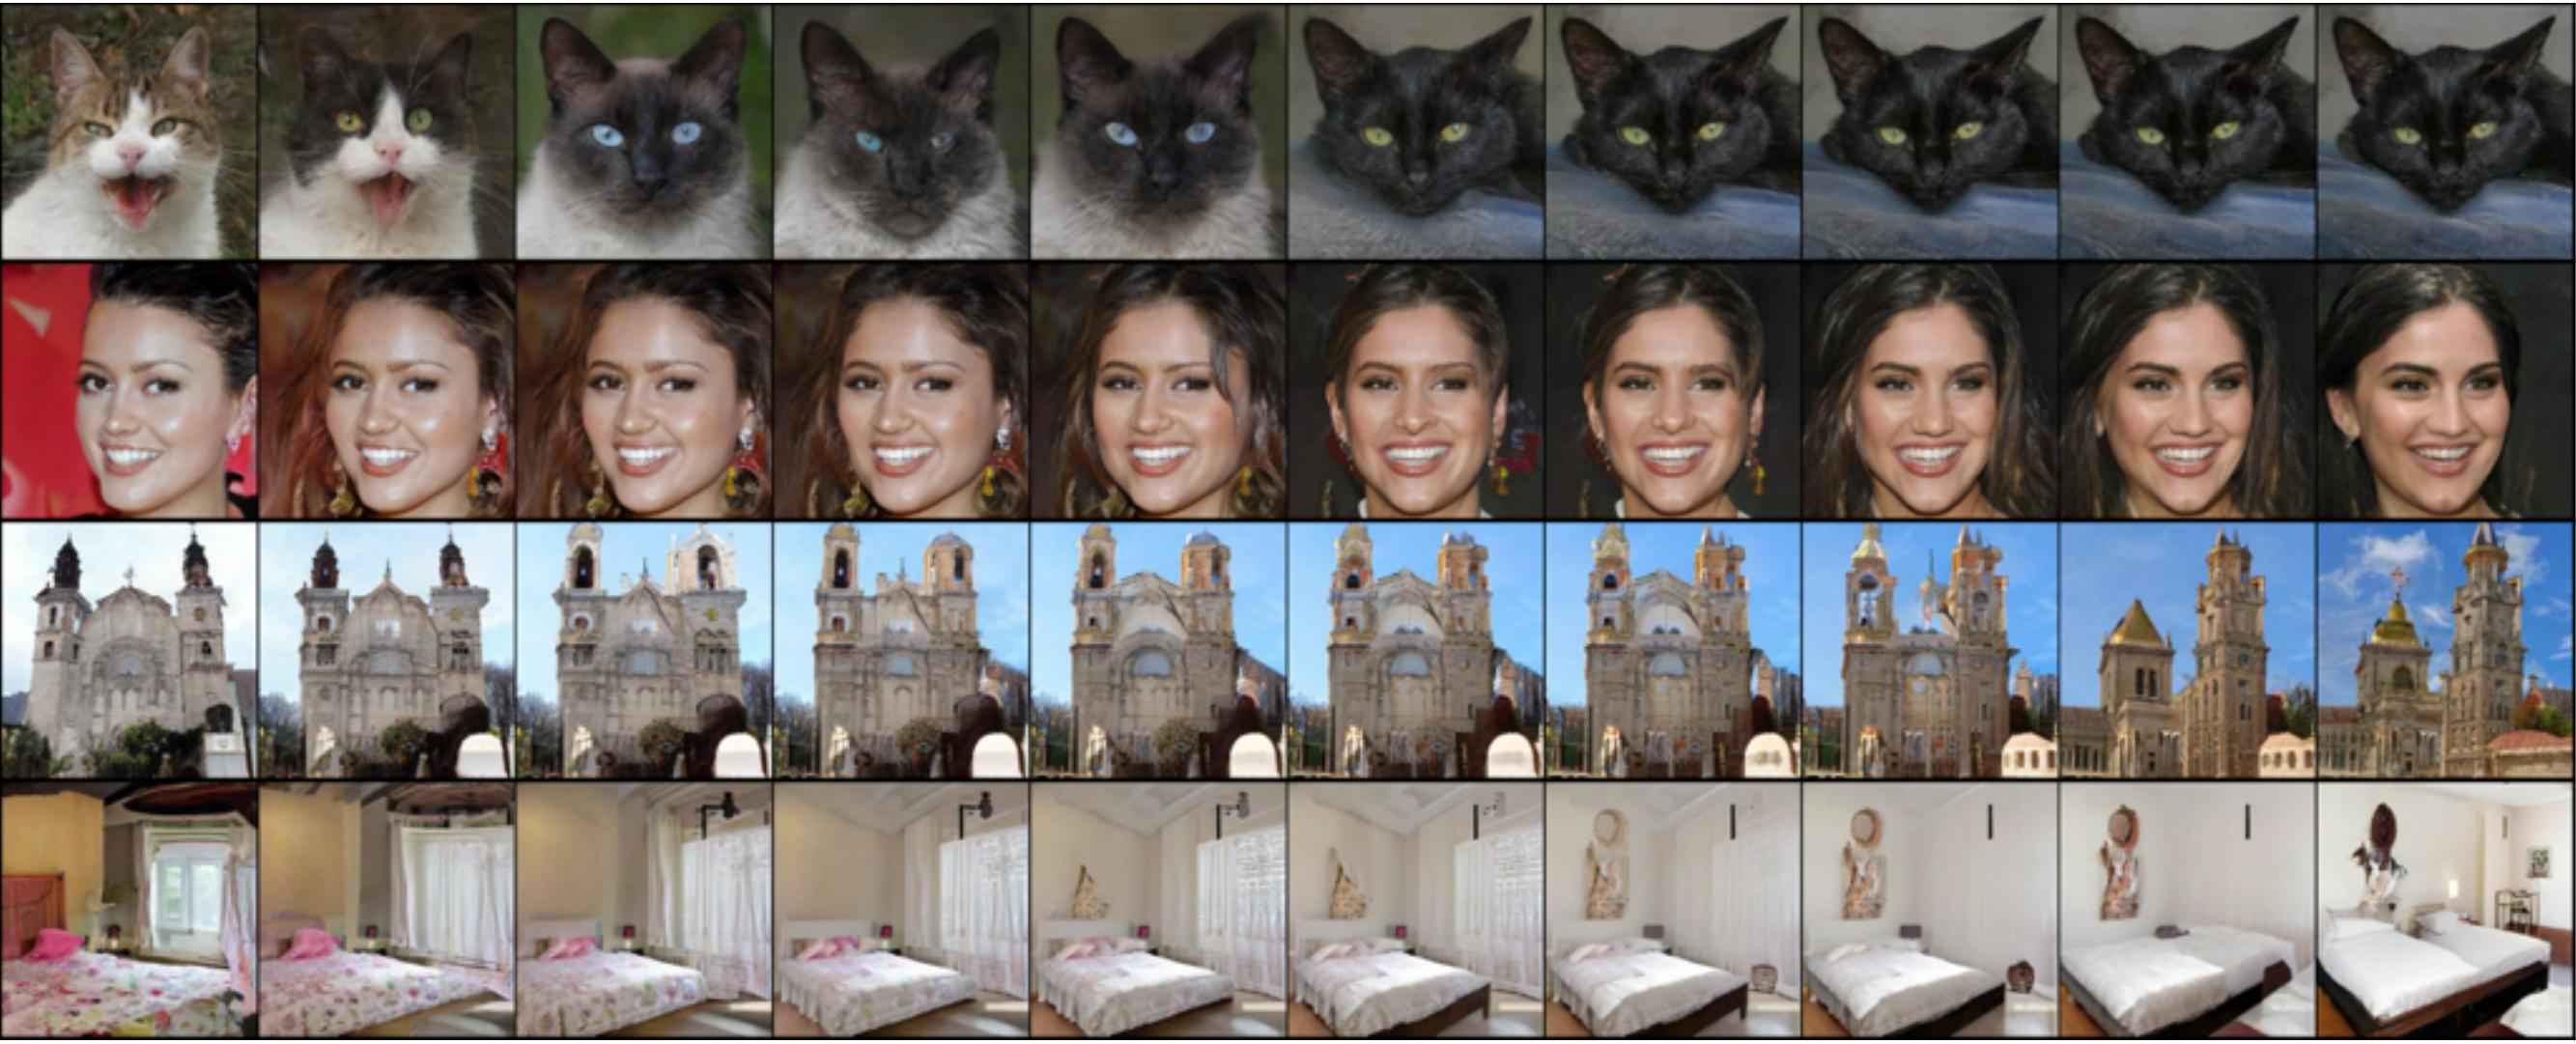
\includegraphics[width=0.95\textwidth]{arxiv_figures/latent_space_interp.jpeg}
    \caption{
    To visualize the latent space, we randomly sample $z_0$ and $z_1$ from $\mathcal{N}(0, I)$, and show the generated images of $\sqrt{\alpha} z_0 + \sqrt{1- \alpha} z_1$ for $\alpha \in [0,1]$.
    }
    \label{fig:interp}
\end{figure}

\begin{figure}
    \centering
    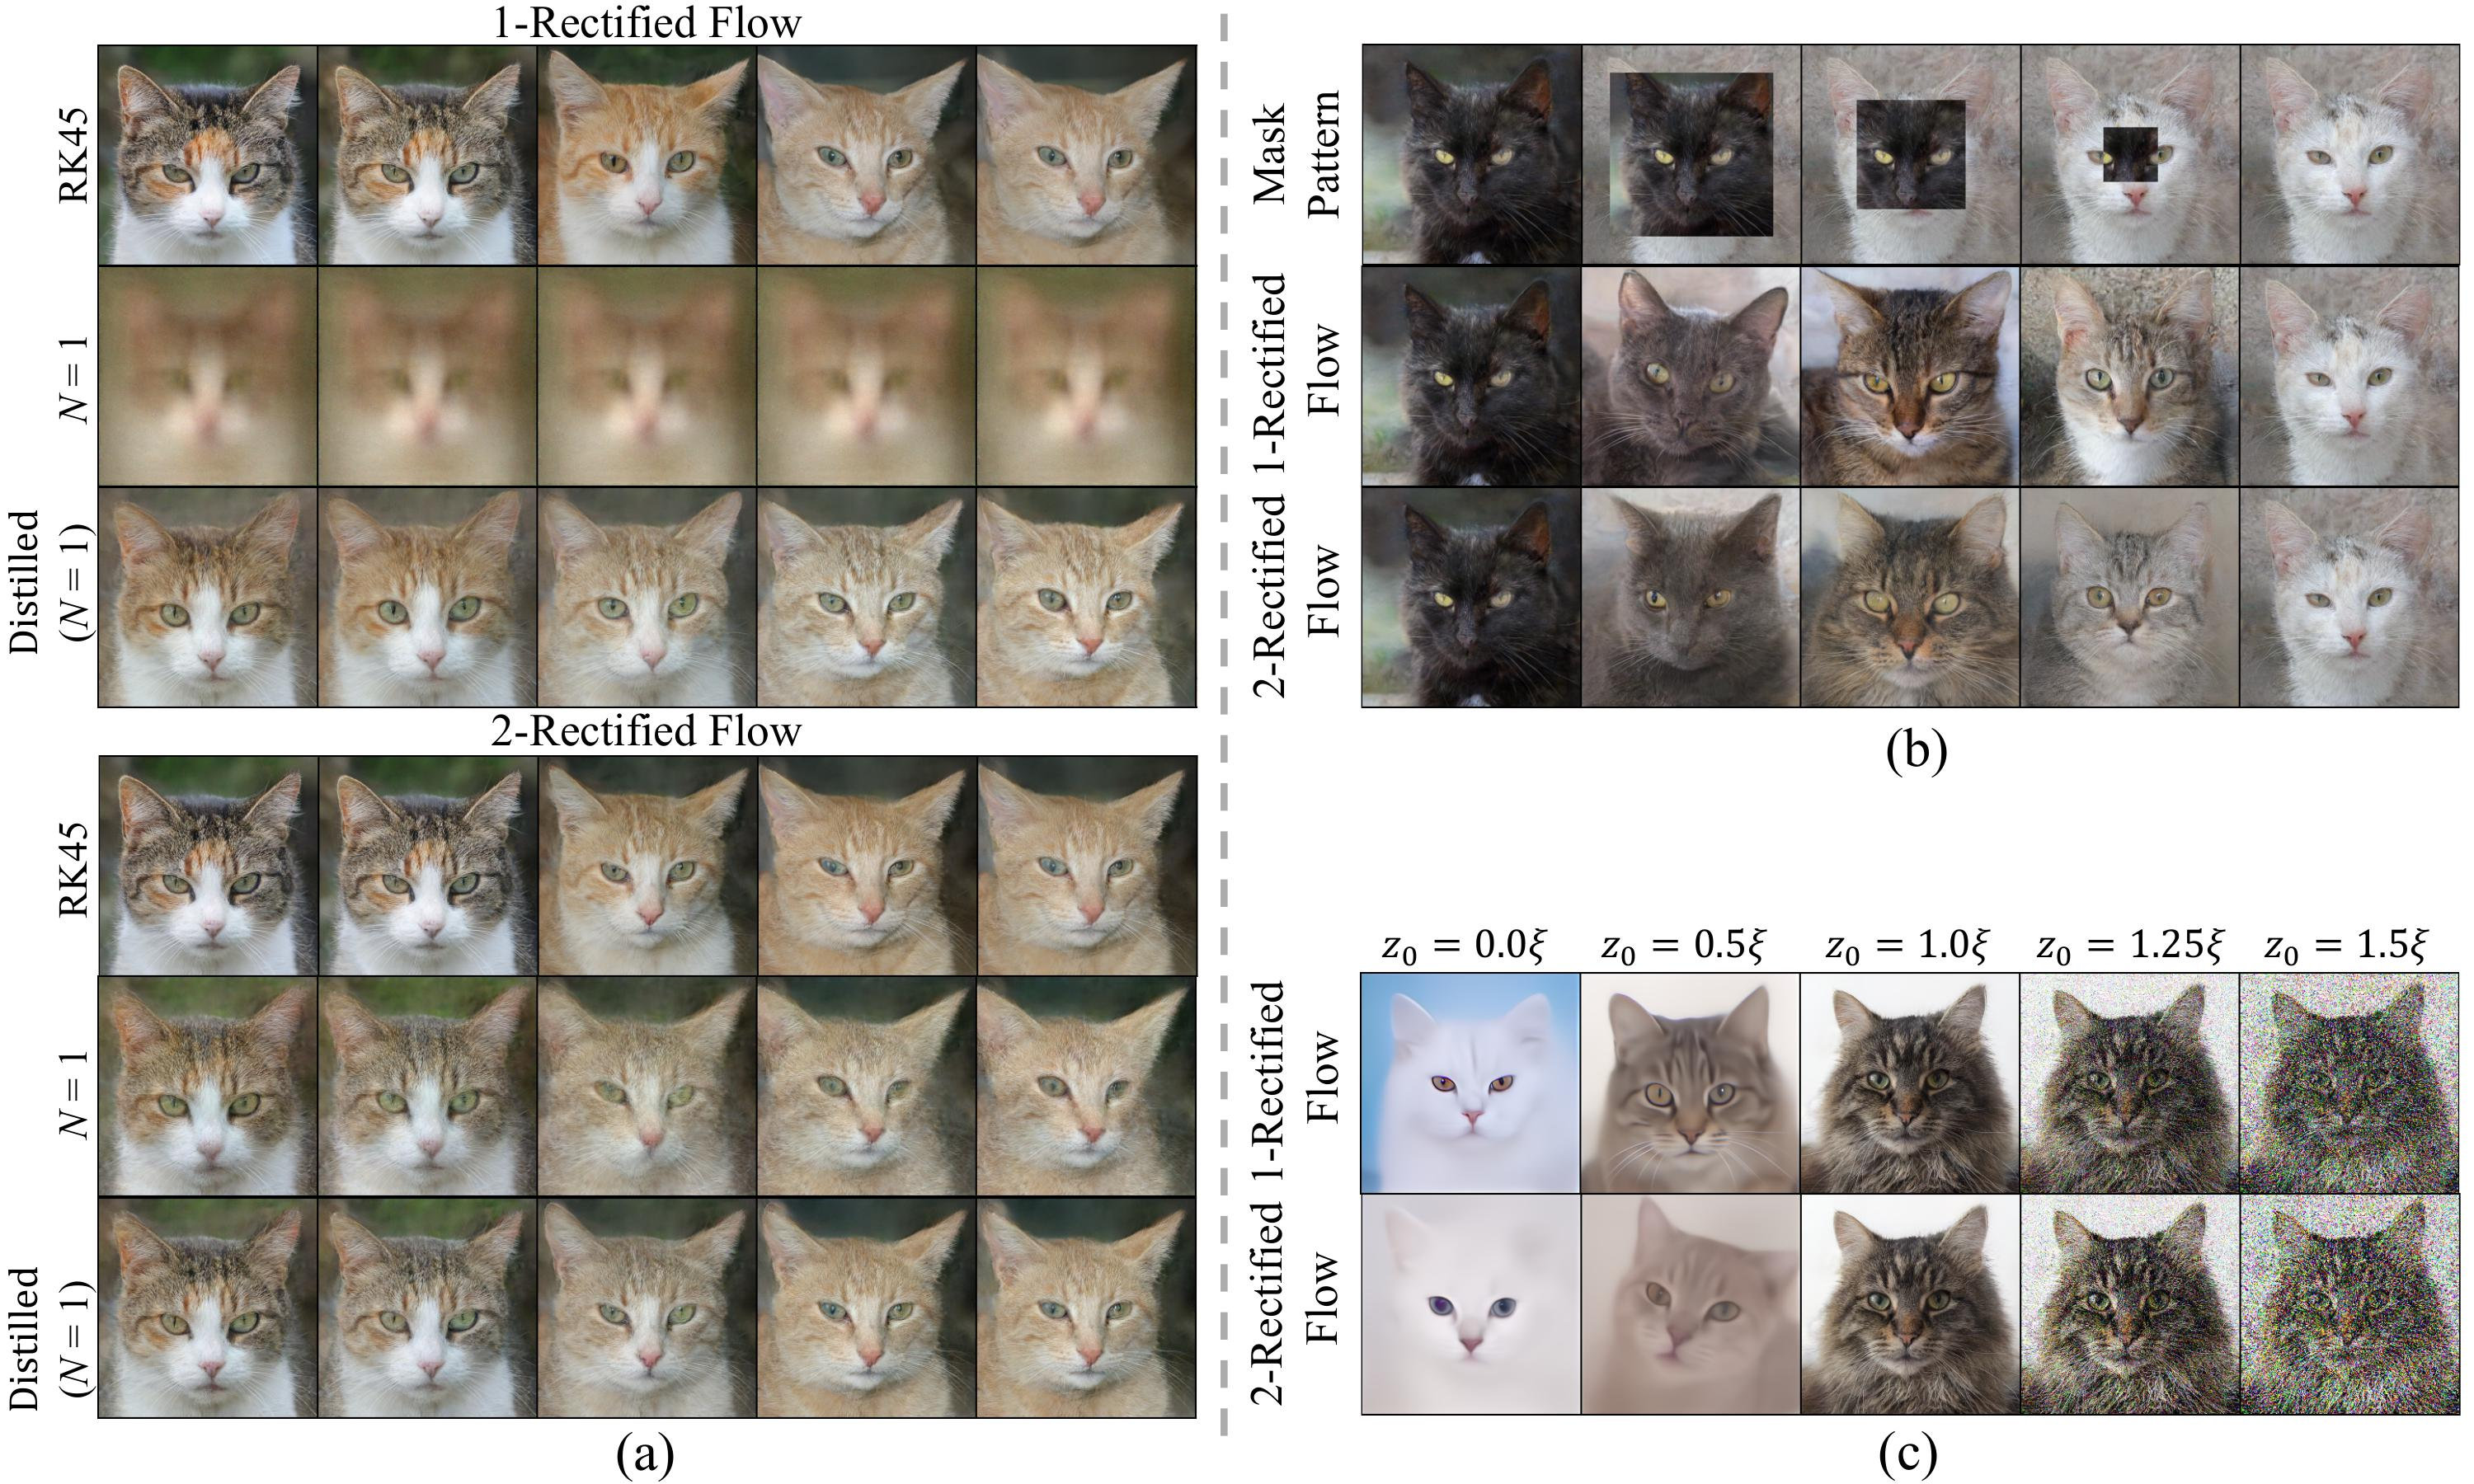
\includegraphics[width=0.98\textwidth]{arxiv_figures/latent_interp_combine.jpeg}
    \caption{
    (a) We compare the latent space between Rectified Flow (0) and (1) using different sampling strategies with the same random seeds. We observe that (i) both 1-Rectified Flow and 2-Rectified Flow can provide a smooth latent interpolation, and their latent spaces look similar; (ii) when using one-step sampling ($N=1$), 2-Rectified Flow can still provide visually recognizable interpolation, while 1-Rectified Flow cannot; (iii) Distilled one-step models can also continuously interpolate between the images, and their latent spaces have little difference with the original flow.
    (b) We composite the latent codes of two images by replacing the boundary of a black cat with a white cat, then visualize the variation along the trajectory. The black cat turns into a grey cat at first, then a cat with mixing colors, and finally a white cat.
    (c) We randomly sample $\xi \sim \normal(0, I)$, then generate images with $\alpha \xi$ to examine the influence of $\alpha$ on the generated images. We find $\alpha<1$ results in overly smooth images, while $\alpha > 1$ leads to noisy images. 
    }
    \label{fig:interp_combine}
\end{figure}

\begin{figure}
    \centering
    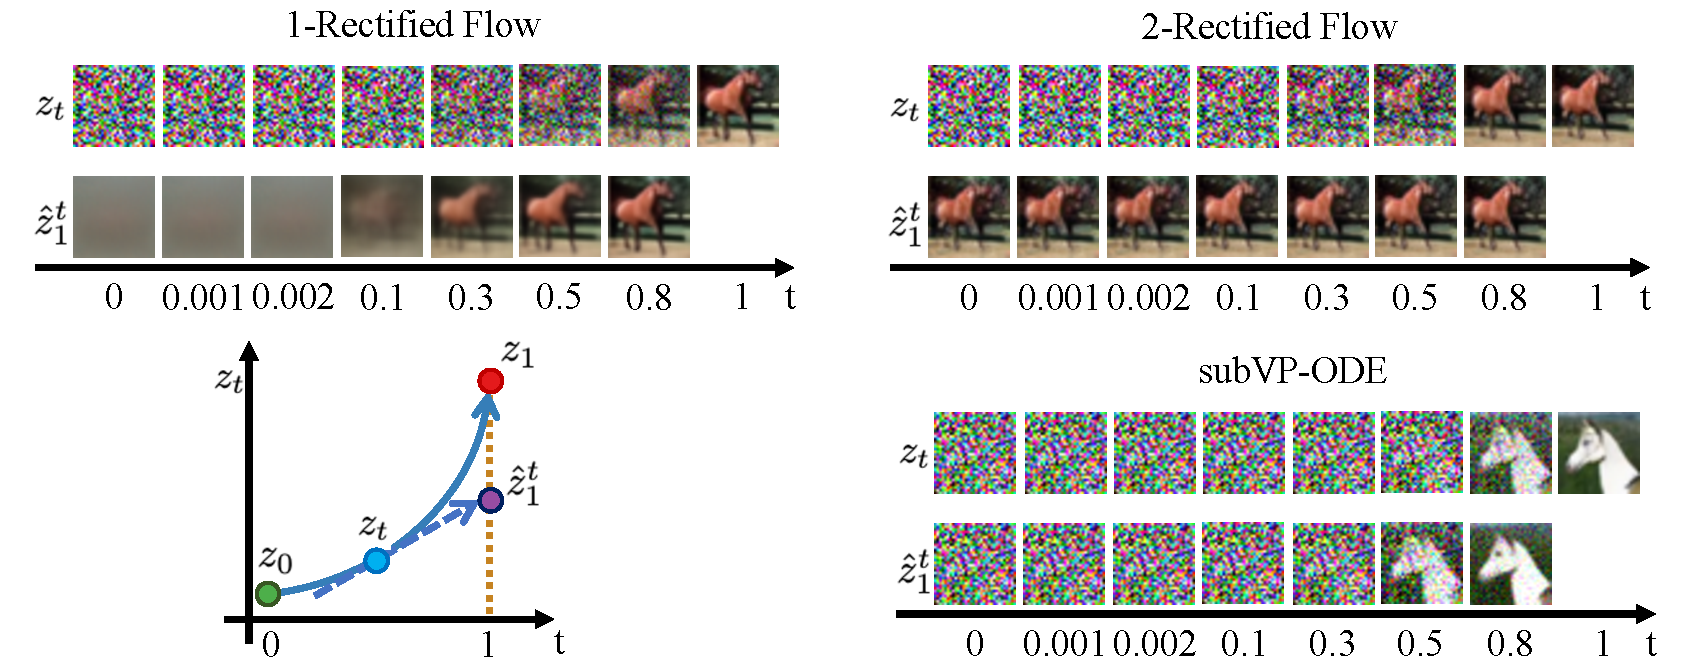
\includegraphics[width=0.98\textwidth]{arxiv_figures/flow_target_comparison.pdf}
    \caption{
    Sample trajectories $z_t$ of different flows on the CIFAR10 dataset,  %
    and the extrapolation $\hat{z}_1^t =z_t + (1-t) v(z_t, t)$ from different $z_t$. The same random seed is adopted for all three methods. The $\hat z_1^t$ of 2-rectified flow is almost independent with $t$, indicating that its trajectory is almost straight. 
    }
    \label{fig:cifar_target}
\end{figure}


\begin{figure}
    \centering
    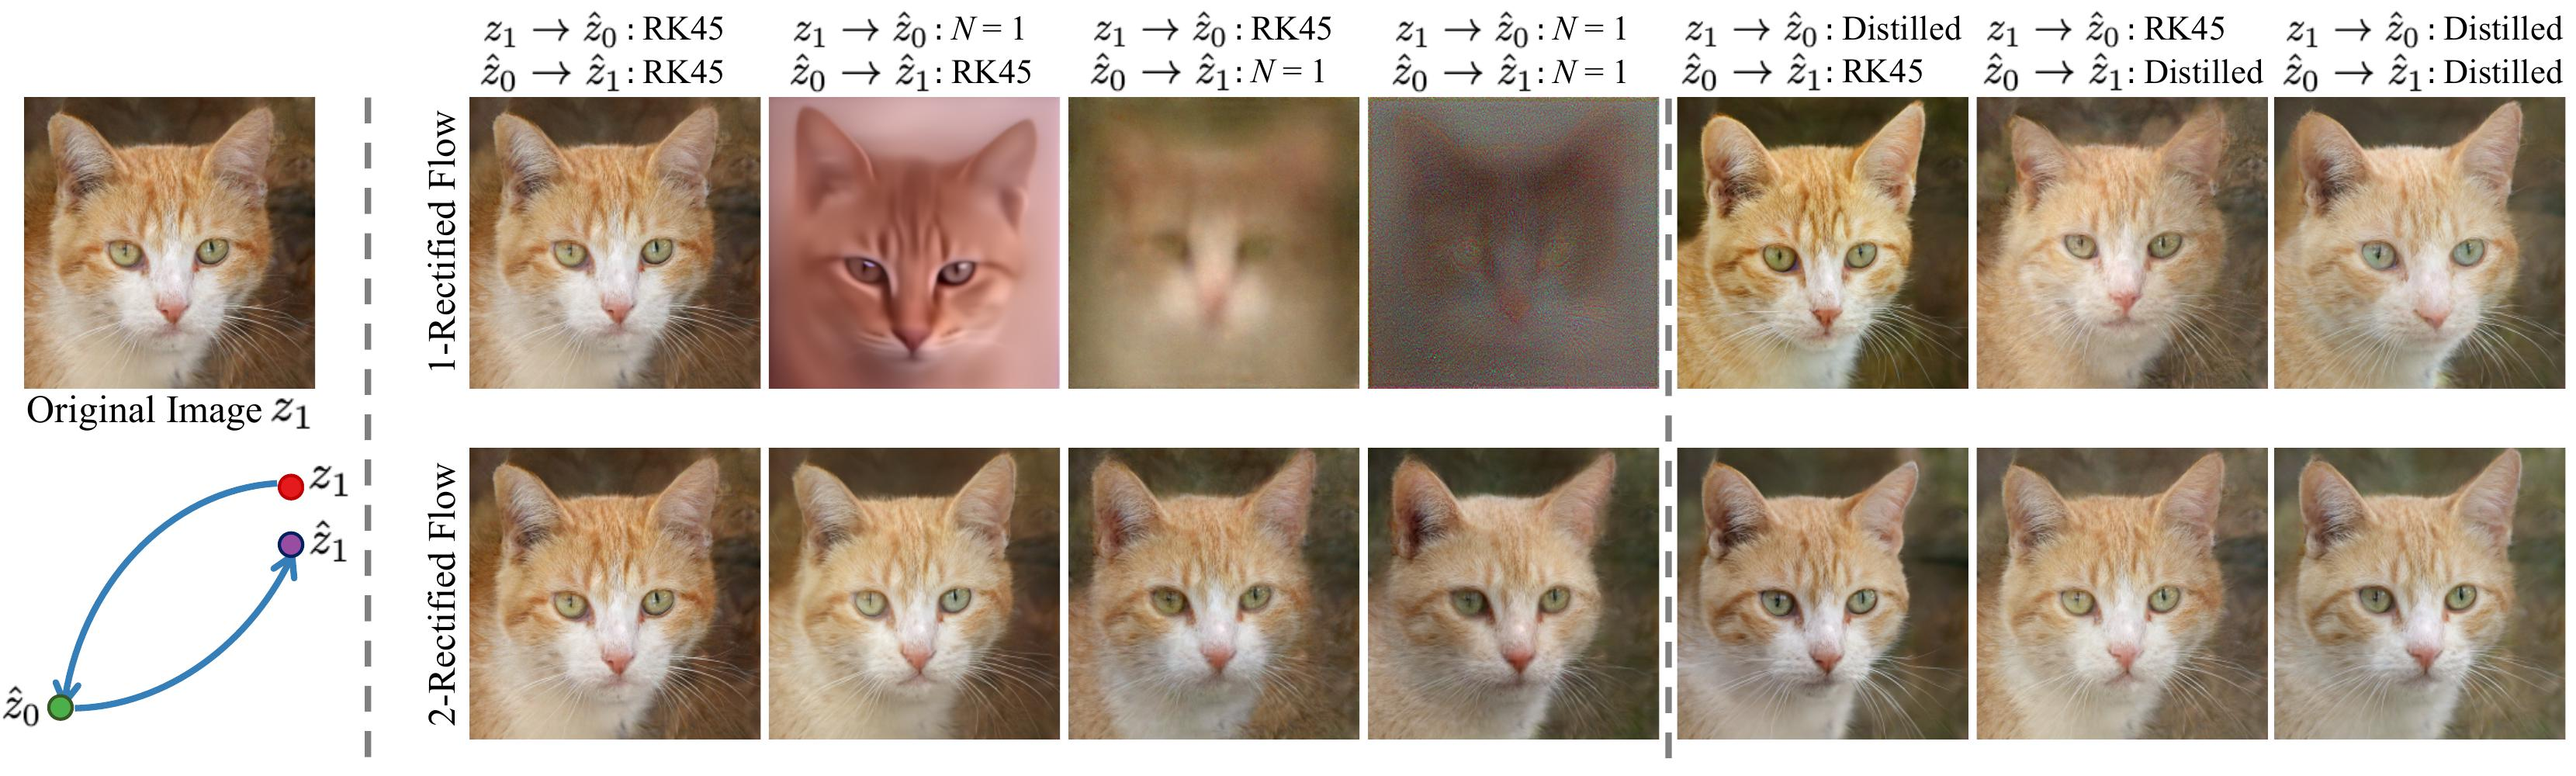
\includegraphics[width=0.95\textwidth]{arxiv_figures/image_reconstruction_new.jpeg}
    \caption{
    We perform latent space embedding / image reconstruction here. Given an image $z_1$, we use an \emph{reverse ODE solver} to get a latent code $\hat{z}_0$, then use a \emph{forward ODE solver} to get a reconstruction $\hat{z}_1$ of the image. The columns in the figure are \emph{reverse ODE solver (forward ODE solver)}. (i) Thanks to the`straightening' effect, 2-rectified flow can get meaningful latent code with only one reverse step. It can also generate recognizable images using one forward step. 
    (ii) With the help of distilled models, one-step embedding and reconstruction is significantly improved. 
    }
    \label{fig:image_reconstruction}
\end{figure}

\begin{figure}[h]
    \centering
    \includegraphics[width=\textwidth]{arxiv_figures/traj1.pdf} \\ 
    \includegraphics[width=\textwidth]{arxiv_figures/traj2.pdf}\\
    \includegraphics[width=\textwidth]{arxiv_figures/traj3.pdf}
    \caption{
    More results for image-to-image translation between different domains. 
    The images in each row are time-uniformly sampled from the trajectory of 1-rectified flow solved $N=100$ Euler steps with constant step size. 
    }
    \label{fig:appendix-traj1}
\end{figure}



